\chapter{Implementación de la solución}

Este capítulo detalla la implementación del algoritmo evolutivo desarrollado. Comienza describiendo a la biblioteca utilizada Malva y continua especificando el algoritmo evolutivo desarrollado donde se explica: la representación del cromosoma, la generación de la población, la función de \emph{fitness} y el funcionamiento de los operadores evolutivos. Para finalizar se detalla el modelo de paralelismo utilizado.

\section{Implementación: Biblioteca Malva}

Dada la complejidad del problema, se contempló desde el inicio del proyecto la utilización de un \emph{framework} para el desarrollo del algoritmo evolutivo. De esta forma, se logra una implementación robusta y flexible. 

Como se detalló en el marco teórico, existen varias opciones disponibles para seleccionar un \emph{framework} para AEs. Por las particularidades del problema planteado, existen ciertos requerimientos a la hora de seleccionar un \emph{framework}, entre los que se destacan:

\begin{itemize}
	\item Código abierto y gratuito: Al ser un proyecto de investigación de índole académico es conveniente que no existan costos económicos asociados. Además, es importante que se cuente con el código abierto con el fin de introducir modificaciones en el código base o corregir errores.
	\item Algoritmo genético: El \emph{framework} debe facilitar el desarrollo de un algoritmo genético ya que es la base en la que se sustenta el proyecto.
	\item Algoritmo paralelo: Por la complejidad del problema y el alto consumo de recursos computacionales que insume el proceso de evaluación de solciones utilizando simulaciones de SUMO, es fundamental que el \emph{framework} incluya la opción de ejecución en paralelo. Si no cuenta con esta funcionalidad nativa, es deseable al menos que exista la posibilidad de modificar el código base para agregarla.
	\item Plataforma: Es requerido que el \emph{framework} se pueda ejecutar en la plataforma de computación de alto desempeño Cluster FING cuyo sistema operativo es Linux CentOs, ya que es donde se realiza el análisis experimental del trabajo. 
	\item Confiabilidad: Es deseable que el \emph{framework} sea lo suficientemente estable como para tener confianza de que el algoritmo funcionará de manera correcta. Se valorará muy positivamente que existan casos de éxito usando el \emph{framework}, la existencia de documentación accesible, ejemplos de código desarrollado, etc.
	\item Lenguaje: Es deseable que el framework esté desarrollado en C++ o Java ,por la experiencia que el equipo de desarrollo cuenta en estos lenguajes. 
	\item Multiobjetivo: Es deseable (aunque no requerido) que el framework soporte algoritmos multiobjetivo; no es requerido porque la función que se quiere implementar es sencilla y puede usarse una agregación lineal de los objetivos.
\end{itemize} 

Luego de analizar los puntos anteriores, se seleccionó la biblioteca Malva para la implementación del algoritmo evolutivo. Malva cumple con la mayoría de los puntos: es de código abierto y gratuito, facilita el desarrollo un algoritmo genético, funciona en la plataforma Cluster Fing, utiliza el lenguaje C++ y el punto de mayor peso en la decisión fue la confiabilidad que daba saber que ya se habían realizado implementaciones exitosas de soluciones similares utilizando algoritmos evolutivos paralelos en la plataforma Cluster Fing. Los dos puntos donde Malva no satisface totalmente el requerimiento son: el funcionamiento en paralelo y el soporte de algoritmos multiobjetivo. Estos problemas se pueden resolver de forma aceptable y sencilla como se explica a continuación. Para el caso del funcionamiento en paralelo al ser Malva de código abierto, es posible modificar el código para soportar la creación de hilos de ejecución, este procedimiento se explica en mas detalle en la ultima sección de este capítulo que trata sobre el modelo de paralelismo y su implementación. El segundo punto acerca del soporte de algoritmos multiobjetivo por parte del \emph{framework}, no supone un gran inconveniente, ya que la función de \emph{fitness} que se plantea utilizar es una combinación lineal sencilla de objetivos y puede ser utilizada en Malva. A continuación se detalla su funcionamiento y características.

Como se explicó anteriormente, Malva \citep {Malva} surge como una variante del proyecto Mallba \citep{Mallba}. Malva propone la actualización, mejora y desarrollo de Mallba como un proyecto de código abierto colaborativo.  Su objetivo es proveer varios esqueletos de heurísticas de optimización que puedan ser utilizados y extendidos de manera fácil y eficiente. Los esqueletos se basan en separar dos conceptos: el problema concreto que se quiere resolver y el método utilizado para resolverlo. Por lo tanto, un esqueleto se puede ver como una instancia de una plantilla genérica para resolver un problema particular, manteniendo todas las funcionalidades genéricas.

Malva utiliza el lenguaje C++, con el objetivo de brindar modularidad y flexibilidad. Los esqueletos se ofrecen como un conjunto de clases \emph{requeridas} que el usuario deberá modificar para adaptarlo a su problema, y clases \emph{provistas} que incluyen todos los aspectos internos del esqueleto siendo  independientes del problema particular. Entre los algoritmos provistos se encuentran los algoritmos genéticos,algoritmo  CHC \citep{CHC} y otros.


\section{Especificación del Algoritmo Genético utilizado}
Se utiliza el algoritmo genético provisto por la biblioteca  Malva llamado "NewGA", con las modificaciones detalladas en la sección anterior. El siguiente esquema describe el funcionamiento del algoritmo utilizado:

\begin{algorithm}[H]
	\caption{Algoritmo Genético de Malva. }
	\label{alg:algoritmo_genetico_malva}
	\begin{algorithmic} [1] 
		{
			\STATE \texttt{t} = 0
			\STATE {Inicializar( P(t))}
			\STATE {Evaluar estructuras en ( P(t))}			
			\WHILE {\text{No terminar}}
			\STATE \texttt{t}++		
			\STATE {Seleccionar C(t) de P(t-1)}	
			\STATE {Recombinar estructuras en C(t) formando C'(t)}				
			\STATE {Mutar estructuras en C'(t) formando C''(t)}		
			\STATE {Evaluar estructuras en C''(t) generando un hilo de ejecucion por cada una}					
			\STATE {Consolidar valores de la evaluacion}								
			\STATE {Reemplazar P(t) de C''(t) y P(t-1)}								
			\ENDWHILE
		}
	\end{algorithmic}
	
\end{algorithm}

A continuación se realiza un resumen de las características del algoritmo implementado, que en la siguiente sección serán descritas en detalle:
\begin{itemize}
	
	\item Se aplica un modelo de algoritmo evolutivo paralelo, utilizando el esquema maestro-esclavo, donde en cada iteración el maestro genera un hilo por cada evaluación de la función de \emph{fitness} y luego espera a la terminación de todos los hilos para consolidar los datos. 
	\item Se considera una formulación multiobjetivo del problema, que intenta optimizar tanto la velocidad promedio de vehículos como la de ómnibus, teniendo cada componente un peso específico en la combinación lineal utilizada para definir la función de \emph{fitness}.
	\item La representación de soluciones: es un vector de números naturales, que representan la duración de las fases de los semáforos y el \emph{offset} para todos los semáforos del Corredor Garzón.
	\item Respecto a los operadores evolutivos: se implementa una variante del cruzamiento de un punto específico para este problema y se utilizan dos tipos de mutación para modificar la duración de fase y el \emph{offset} de los semáforos.
	\item Respecto a los criterios de selección y reemplazo el AE propuesto utiliza un modelo generacional y reemplaza padres por hijos. La selección de los padres se realiza por el método de torneo de tres individuos y la selección de hijos por el método de selección proporcional.
	
\end{itemize}

\subsection{Representación de individuos}

Como se explicó en el marco teórico, el problema de sincronización de semáforos puede ser resuelto optimizando diferentes parámetros. Entre estos parámetros se encuentran la duración de fase, de ciclo y el \emph{offset} de los semáforos. Los parámetros que se seleccionen deberán ser incluidos en la representación del cromosoma.

Para la solución propuesta se contempla tanto la duración de fase como el \emph{offset}. La figura \ref{fig:cromosoma1} muestra la representación del cromosoma, como se puede observar se agrupa lógicamente en cruces, siendo el valor de cada gen la duración de una fase en un cruce. Además, se agrega para cada cruce el valor del \emph{offset}. Se utiliza un vector de números naturales para favorecer la claridad en el desarrollo y la facilidad a la hora de aplicar los operadores. Por este motivo el tamaño del cromosoma depende de la cantidad de cruces y de la cantidad de fases que incluya cada cruce. Con esta representación se busca una optimización global de todo el sistema y no individualmente para cada cruce, lo cual es fundamental para mejorar la velocidad promedio del Corredor Garzón y del resto de las calles que lo cruzan.

\begin{figure}[H]
	\centering
	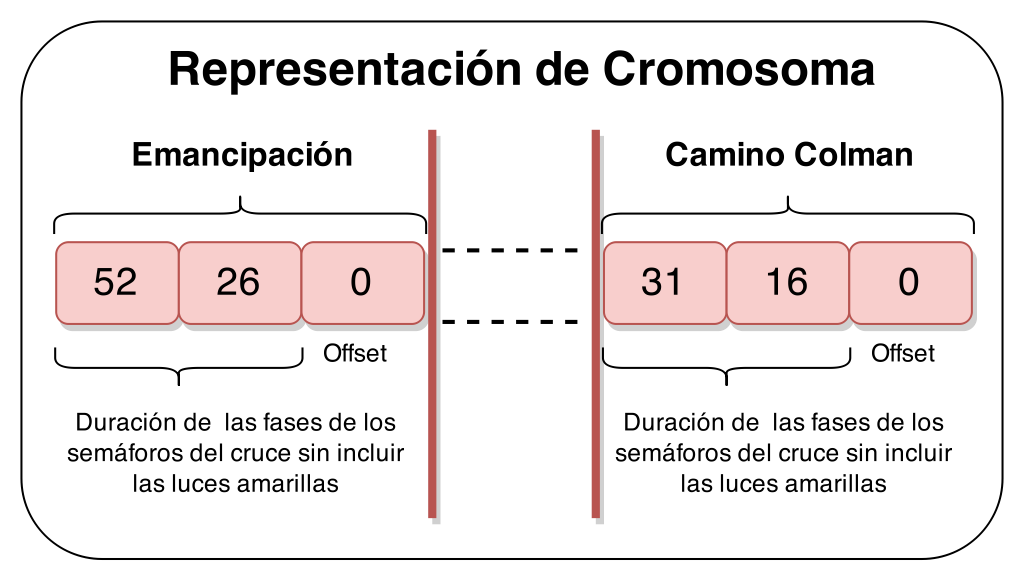
\includegraphics[width=0.8\linewidth]{Figures/cromosoma1}
	\caption{Vista del Cromosoma para los cruces de Avda. Millán y Cno. Ariel}
	\label{fig:cromosoma1}
\end{figure}

Toda la información del cromosoma se guarda y carga en el formato \emph{XML}, del archivo de configuración de semáforos, que utiliza el simulador SUMO. La Figura \ref{fig:rep_sumo} muestra como se modela la esquina de Garzón y Emancipación en el formato antes mencionado. Para las distintas fases o secuencias de luces de los semáforos de una determinada esquina, se utiliza la etiqueta \emph{phase}, donde \emph{state} contiene información sobre la secuencia de luces, por ejemplo, la fase \emph{GGGGrrrGGGGrrr} indica la secuencia de luces, \emph{G} indica la luz verde con preferencia, \emph{g} indica la luz verde sin preferencia, \emph{r} la luz roja, \emph{y} luz amarilla; y  \emph{duration} especifica la duración de la fase, que corresponderá a los alelos de duraciones del cromosoma,  en la representación del cromosoma se omiten las fases que contengan luces amarillas ya que no modifican los tiempos reales del paso de vehículos. El tiempo indicado en el \emph{offset} especifica el inicio de la fase y será el correspondiente al del gen de Emancipación.


\begin{figure}[H]
	\centering
	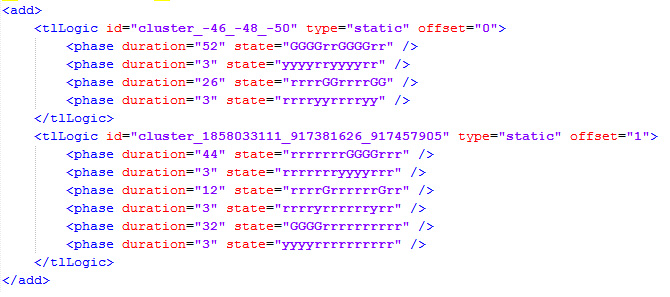
\includegraphics[width=\linewidth]{Figures/rep_sumo}
	\caption{Representación de Sumo}
	\label{fig:rep_sumo}
\end{figure}



\newpage

\begin{figure}[H]
	\centering
	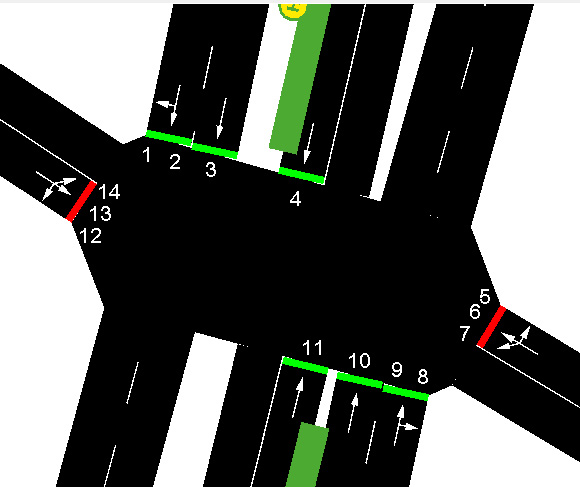
\includegraphics[width=0.7\linewidth]{Figures/semaforos_numerado}
	\caption[Representación de una fase de los semáforos para un cruce.]{Representación de una fase de los semáforos para un cruce. Cada número se corresponde a una letra en la secuencia de \emph{state} del archivo de configuración del simulador SUMO.}
	\label{fig:sem_numerados}
\end{figure}
El simulador representa en las esquinas, mediante el uso de flechas blancas, la elección de carriles habilitados, para los vehículos que transitan por un determinado carril; en el caso de un giro, la flecha apunta hacia donde se encuentra el carril del giro. La figura \ref{fig:sem_numerados} muestra como se modela la esquina de Garzón y Emancipación en el simulador, se le añadieron los números del 1 al 14 para indicar todas las flechas blancas de la esquina y establecer la correspondencia con la figura \ref{fig:rep_sumo}. Por tanto para el estado \emph{GGGGrrrGGGGrrr} se tiene que:
\textit{i)} \emph{GGGG} se corresponde a 1, 2, 3 y 4, \textit{ii)} \emph{rrr} se corresponde a 5, 6 y 7, \textit{iii)} \emph{GGGG} se corresponde a 8, 9, 10 y 11. y \textit{iv)}\emph{rrr} se corresponde a 12, 13 y 14. Estableciendo esta correspondencia para cada cruce, se modelan las secuencias y duraciones de luces originales de manera que represente lo relevado in situ.


\subsection{Generación de la población inicial}

Para la inicialización de la población se toma como referencia
la configuración obtenida a partir de los datos de la realidad, recolectadas en el relevamiento realizado. Luego, para cada cruce se varían las duraciones de las fases de manera aleatoria entre un rango de valores configurable. Además, la fase inicial se selecciona aleatoriamente entre la cantidad de fases del cruce.

\subsection{Función de \emph{fitness}}


La evaluación de un individuo se realiza generando un archivo de texto con la configuración de los semáforos en base a su cromosoma y ejecutando el simulador SUMO para obtener un archivo de salida con los datos necesarios para calcular el \emph{fitness} (como la velocidad promedio de ómnibus y otros vehículos).

Se emplea una función multiobjetivo usando combinación lineal de la velocidad de los ómnibus y del resto de los vehículos.
%ya que es un método sencillo y adecuado cuando el problema de optimización involucra menos de tres objetivos y el frente de Pareto del problema es convexo \citep{coello2002evolutionary}. 
El \emph{fitness} se calcula como una suma ponderada, con los pesos fijados a priori, de acuerdo a la expresión en la Ecuación \ref{eq:funcion_fitness_generica}.

\begin{equation}
\label{eq:funcion_fitness_generica}
F(x) = \sum_{i=1}^{n}{w_i}{f_i}(x)
\end{equation}

Se seleccionan como objetivos la velocidad promedio de los ómnibus (vpb) y la velocidad promedio del resto de los vehículos (vpv). Estos objetivos fueron elegidos ya que son  adecuados para realizar las comparaciones con la realidad, ya que las velocidades promedio se pueden obtener simulando las instancias que representan la realidad. Otros objetivos podrían utilizarse, como la cantidad de vehículos que completan su viaje, la duración promedio del recorrido o el tiempo de simulación pero no son útiles para realizar comparaciones con la realidad ya que son datos que no se pueden medir u obtener con facilidad.

La función de \emph{fitness} utilizada se presenta en la Ecuación \ref{eq:funcion_fitness}, donde \emph{$w_1$} e \emph{$w_1$} indican los pesos que se especifican en la función. En una primera instancia se establece $w_1$ = $w_2$ = 1, más adelante se experimentará con otros pesos.

\begin{equation}
\label{eq:funcion_fitness}
f = w_1.vpb + w_2.vpv
\end{equation}



Se plantea optimizar la velocidad promedio de los vehículos en toda la red vial (vpv), de manera global, esto quiere decir que se busca una mejor velocidad promedio tanto en autos que van por Garzón como aquellos que circulan por el resto de las calles del escenario geográfico estudiado. Por este motivo cuando se realicen las simulaciones de las instancias realistas del problema se tendrán en cuenta las velocidades promedio de todos los vehículos participantes, cuyo valor sera utilizado en la función de \emph{fitness} (variable vpv). La optimización global es fundamental para lograr una mejora en la velocidad promedio de toda la red vial, ya que si cada cruce se optimiza individualmente podría generar problemas de congestión en otras zonas.

\subsection{Operadores Evolutivos}

\subsubsection{Operador de Cruzamiento}
Se utiliza cruzamiento de un punto, seleccionando del cromosoma una posición aleatoria entre dos cruces como punto de corte, motivado por el hecho de que si un tramo del corredor tiene un buen comportamiento, se intenta mantener esa propiedad. En el escenario que plantea la Figura \ref{fig:op_cruzamiento}, los padres cuentan con tres cruces. Se elige un punto de corte aleatoriamente entre dos cruces, cortando a los padres e intercambiando los trozos del cromosoma para generar los hijos como se ve en la Figura \ref{fig:op_cruzamiento} .


\begin{figure}[H]
	\centering
	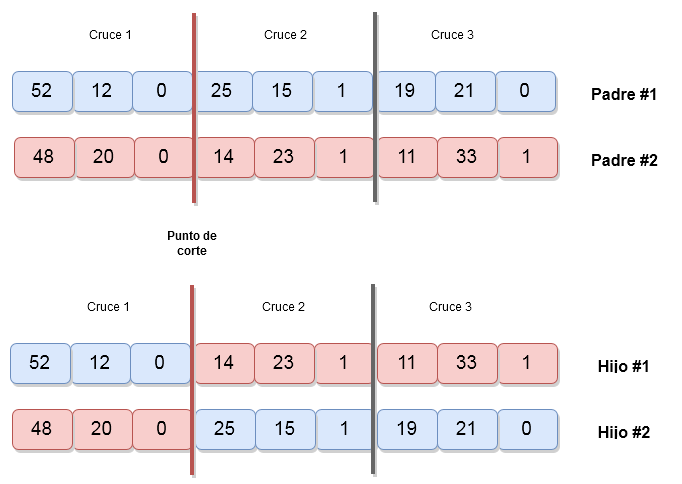
\includegraphics[width=0.8\linewidth]{Figures/alg_cruzamiento}
	\caption{Ejemplo del operador de cruzamiento utilizado}
	\label{fig:op_cruzamiento}
\end{figure}



\subsubsection{Operador de Mutación}
Se implementaron dos tipos de mutación:
\begin{itemize}
	
	\item Mutación de duración de fase: para cada fase de cada cruce se modifica su duración sumando o restando una cantidad dada de segundos. Se valida que el nuevo valor obtenido se encuentre dentro de un rango especificado de entre 5 y 60 segundos (valores que se pueden modificar), para que no se produzcan casos alejados de la realidad, por ejemplo una intersección donde los vehículos tengan menos de 5 segundos para cruzar.
	
	\item Mutación del \emph{offset}: Para cada \emph{offset} del cromosoma se suma o resta una cantidad de segundos dada y se valida que esté dentro de un rango prefijado de entre 0 y el máximo valor de \emph{offset} para ese cruce.
	

\end{itemize}
Ambas mutaciones son aplicadas de acuerdo a una tasa de probabilidad prefijada.

\subsubsection{Selección y reemplazo}
Se  utilizan los operadores y criterios provistos por el algoritmo genético newGA de Malva. La selección de padres se realiza por el método de torneo de tres individuos y la selección de hijos por el método de selección proporcional. 

Malva incluye dos políticas de reemplazo, la primera indica que se reemplazan padres por hijos y la segunda que solamente los nuevos hijos pueden ser padres, para el algoritmo evolutivo propuesto se utiliza la primera opción por lo que tanto padres como hijos pueden ser parte de la siguiente generación.

\subsubsection{Parámetros del algoritmo}
Los parámetros del algoritmo son: el número de generaciones que se realizan hasta detener el algoritmo, el tamaño de la población que indica la cantidad de individuos incluidos en el algoritmo evolutivo, la tasa de probabilidad de cruzamiento y de mutación que se utiliza para determinar cuando aplicar los operadores de cruzamiento y mutación. Los valores específicos de los parámetros del algoritmo evolutivo se ajustan en el capítulo 5 donde se realiza el análisis de configuración paramétrica. 

\section{Modelo de paralelismo e implementación}


%The skeletons in MALLBA offer support for parallelism using the distributed memory approach (i.e., implementing distributed subpopulation models for metaheuristics). However, the library does not provide support for shared-memory multithreading parallel programming. Multihtreading programming allows implementing efficient algorithms by using multiple threads within a single process. Multihtreading is well suited for multi-core computers, where each thread is executed on a single core. It provides a fast method for concurrent execution; communications and synchronizations are performed via the shared-memory resource, which is handled using mutuallyexclusive operations in order to prevent simultaneous accesses.

%The multithreading master-slave parallel EA proposed in this work was implemented using the GA skeleton in MALLBA. Additional code was incorporated into the GA skeleton to implement several new features:
%– to create and manage the pool of threads used for the fitness evaluation;
%– to implement the master-slave hierarchy and the communications between master and slaves;
%– to define the synchronization mechanisms between threads,
%used to read and write the shared memory. Our implementation starts by creating and initializing a pool of threads to distribute the fitness evaluation. Each thread receives several input parameters from the master process, including the solution to be evaluated, the thread identification, and the index in the array of fitness values.Then, each slave process, implemented in each thread, computes the fitness evaluation by simulating the mobile communications with the proposed


Uno de los requisitos planteados al inicio del presente trabajo era la creación de un algoritmo genético que soportara paralelismo, con el objetivo de reducir los tiempos de ejecución de las simulaciones necesarias para evaluar la función de \emph{fitness} de los individuos. El motivo principal fue que los escenarios planteados se consideraron complejos por lo que la ejecución del algoritmo evolutivo insumiría un tiempo considerable. El código base del algoritmo evolutivo fue modificado para que soportara la ejecución en paralelo. Específicamente, se desarrolló una nueva forma de evaluar a los individuos, generando un hilo de ejecución por cada individuo.

El código del algoritmo genético provisto por la biblioteca Malva (newGA.pro.hh) fue modificado agregando dos nuevas funciones encargadas de llamar a la función de \emph{fitness} y asignar el valor obtenido al individuo tanto para padres (\emph{evaluate{\_}parent{\_}threads}) como hijos (\emph{evaluate{\_}offpring{\_}threads}). En la Figura \ref{fig:codigo1} se presenta el código de la función \emph{evaluate{\_}parent{\_}threads} que se explica a continuación. El parámetro \emph{data} contiene información sobre la población, el individuo a evaluar, su índice y un vector con los valores de \emph{fitness} de la población.
En la línea 378 se hace un chequeo para saber si el valor de \emph{fitness} ya fue obtenido para el individuo, de esta forma no se repiten evaluaciones, en la línea 380 se ejecuta la función de \emph{fitness} y se aplica el valor de \emph{fitness} al individuo, luego en la línea 381 se incrementa el numero de evaluaciones realizadas en la población.
La función \emph{evaluate{\_}offpring{\_}threads} es análoga a \emph{evaluate{\_}parent{\_}threads} pero especifica para los hijos, por lo que no se considera necesario mostrar su código.



\begin{figure}[H]
	\centering
	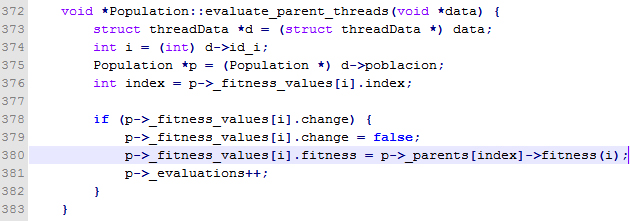
\includegraphics[width=0.99\linewidth]{Figures/codigo1}
	\caption{Nueva función agrega al codigo provisto por Malva.}
	\label{fig:codigo1}
\end{figure}

	
La función \emph{evaluate{\_}parents()} provista por Malva se encarga de iterar sobre los padres de la población y ejecutar la evaluación sobre cada uno de ellos para obtener el valor de \emph{fitness} asociado. Esta función fue modificada para generar un hilo de ejecución por cada evaluación, como se aprecia en la porción de código de la Figura \ref{fig:codigo2}.
En la línea 434  se genera el hilo llamando a la función agregada anteriormente \emph{evaluate{\_}parent{\_}threads}. Luego en la línea 504 se espera a que todos los hilos finalicen su ejecución.
Análogamente se realizan modificaciones similares en la función 	\emph{evaluate{\_}offsprings }que itera sobre los hijos, para que
genere un hilo por cada evaluación de los hijos, llamando a la función de  \emph{evaluate{\_}offpring{\_}threads}.
		
\begin{figure}[H]
	\centering
	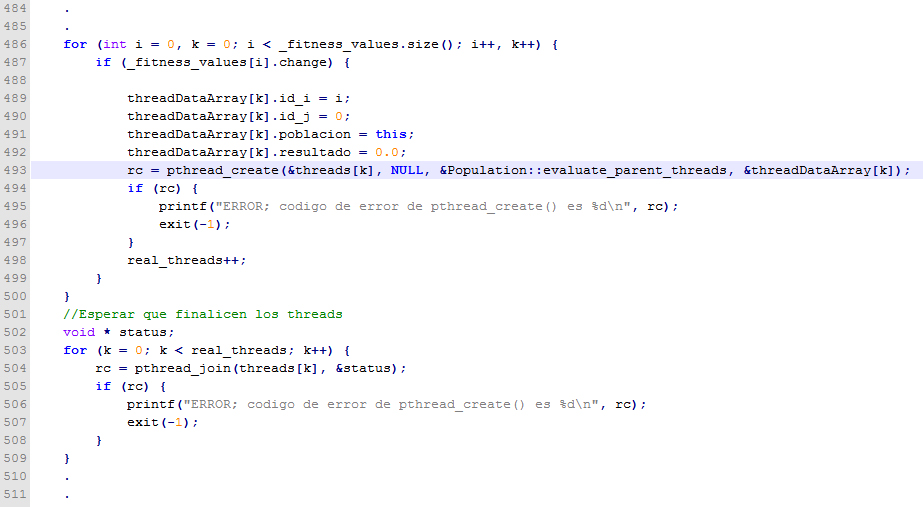
\includegraphics[width=0.99\linewidth]{Figures/codigo2}
	\caption{Modificaciones de la función evaluate{\_}parents.}
	\label{fig:codigo2}
\end{figure}		

Se utilizó el esquema maestro-esclavo para el modelo de paralelismo. El proceso maestro se encarga de la mayoría de las etapas del algoritmo evolutivo, al comenzar, inicializa la población y se encarga de distribuir la evaluación de los individuos hacia los esclavos, creando un hilo de ejecución por cada esclavo. Luego el proceso maestro espera a que las evaluaciones terminen para obtener los valores de \emph{fitness} de los esclavos. Una vez obtenidos los valores, selecciona a los mejores individuos y le aplica los operadores de cruzamiento y mutación. Para finalizar ejecuta el criterio de reemplazo para generar la siguiente población. Mientras, los esclavos se encargan solamente de obtener el individuo enviado por el maestro y de efectuar la evaluación del individuo, que corresponde a ejecutar el simulador y obtener los datos de salida. 


El modelo de paralelismo no cambia el comportamiento del algoritmo secuencial, solo se enfoca en mejorar la eficiencia computacional para poder abordar escenarios realistas y complejos.

En el capítulo siguiente, en la sección de análisis experimental se realiza un estudio de la eficiencia computacional del algoritmo genético paralelo, para comparar los tiempos de ejecución entre la versión paralela y la secuencial.